\documentclass[10pt,twocolumn,letterpaper]{article}
\usepackage[margin=0.7in,columnsep=0.25in]{geometry}
\usepackage{amsmath,amssymb,graphicx,booktabs,caption,placeins}
\makeatletter\newcommand\tabinput[1]{\@@input #1 }\makeatother
\usepackage[numbers,sort&compress]{natbib}
\captionsetup{font=small,labelfont=bf}
\setlength{\parskip}{0pt}
\makeatletter\renewcommand\section{\@startsection{section}{1}{0pt}{-7pt}{2pt}{\normalfont\large\bfseries}}\makeatother
\title{\vspace{-0.6in}\Large The CoE toy model and the Pantheon+ supernovae: what the geometry explains}
\author{Note for Chris, \today}
\date{\vspace{-0.35in}}
\begin{document}
\maketitle
\begin{abstract}\noindent
Your toy model has a real centre of expansion (CoE), gravity as the only force, an always-decelerating expansion and no dark matter, and its purpose is to explain the Migkas cluster anisotropy. We embed it in exact $\Lambda=0$ Lema\^itre--Tolman--Bondi dust models and confront it with the clusters and with the Pantheon+ supernovae (SNe). With the corrected sign $A\propto H_0^2$, your geometry on the CoE axis lowers the cluster $\chi^2$ from 44.7 for isotropy to 20.3. A joint fit to clusters and SNe places the axis $16^\circ$ from the CoE. Among backgrounds, the SNe prefer baryons only, with a free fit giving $\Omega\approx0.068$ and hence about zero dark matter. The SN residuals show no significant anisotropy that conflicts with the CoE axis. Flat $\Lambda$CDM fits the sky-averaged SN distances better, and we give that comparison as context for a model tuned over decades, not as a verdict on the toy model.
\end{abstract}

\section{Question}
Your toy model explains the Migkas et al.\ \cite{Migkas2020,Migkas2021} cluster anisotropy with the tidal field of a large mass toward the CoE. Gravity is the only force, so the expansion always decelerates, and the model contains no dark matter. The CoE mass is unlabelled gravitating mass. The previous note showed that the exact relativistic version of the geometry reproduces the size, $m=2$ shape, axis and sign of the cluster signal. Here we ask what the same geometry does with the Pantheon+ type Ia SN Hubble diagram \cite{Scolnic2022,Brout2022}, which covers the whole sky to high redshift. We lead with what the geometry explains, then give the SN fit quality relative to flat $\Lambda$CDM as context, and then test whether the SN residuals are anisotropic about the CoE.

\section{Models and data}
We use the LTB metric \cite{Bondi1947,Bolejko2011}
\begin{equation}\label{eq:ltb}
\begin{split}ds^2&=-dt^2+\frac{R'^2}{1+2E(r)}\,dr^2+R^2d\Omega^2,\\ \dot R^2&=\frac{2M(r)}{R}+2E(r),\end{split}
\end{equation}
with the solver, bang-time choice and off-centre geodesic code of the previous note. The mass function is an optional uniform background of density parameter $\Omega$ plus your $e^{-r/L}$ CoE mass, which we call the lump and leave unlabelled as to composition, and the observer sits at distance $D$ from its centre with local expansion rate $H_0$. We label the lump by its mass inside $D$ in units of the critical mass,
\begin{equation}\label{eq:mc}
m_c=\frac{2G\,M_{\rm lump}(<D)}{H_0^2D^3},
\end{equation}
so that your best fit has the values in the first row of Table~\ref{tab:par}. We label the backgrounds baryons only, $\Omega=0.05$, which is the preferred physical case for a model without dark matter, and $\Lambda$CDM-equivalent, $\Omega=0.3$, which is the matter density $\Lambda$CDM uses. We also let $\Omega$ float. By the shell theorem (previous note) a uniform background that encloses our visible sphere of radius $R$ only changes the mean expansion rate, matter beyond $D+R$ exerts no net pull, and the anisotropy comes from the net mass inside $D-R$, the core minus the hole swept out of the background,
\begin{equation}\label{eq:mnet}
M_{\rm net}=M(<D-R)-\tfrac{4\pi}{3}\bar\rho\,(D-R)^3>0 ,
\end{equation}
which must be positive for the instantaneous tidal field to put the fastest expansion on the CoE axis. In our LTB models the lump is added on top of the background and the condition is evaluated on the actual evolving density, so $M_{\rm net}$ is the lump mass and is positive by construction. In your time-integrated shell models the history can override the condition, because sources coast through the empty hole feeling only the core (previous note). For each geometry we tabulate the luminosity distance $D_L(z,\psi)$ on Gauss--Legendre nodes in the angle $\psi$ from the lump axis and interpolate to every SN direction.

The data are the Pantheon+ corrected magnitudes $m_{b,\rm corr}$ with the full statistical plus systematic covariance $\mathbf C$, using the peculiar-velocity-corrected redshift $z_{\rm HD}$. Our baseline cut is $z>0.023$, and we repeat the main fits with $z>0.01$. The absolute magnitude and $H_0$ enter only as one additive offset $\mathcal M$, which we remove analytically,
\begin{equation}\label{eq:chi2}
\chi^2=\mathbf r^{\sf T}\mathbf C^{-1}\mathbf r-\frac{(\mathbf 1^{\sf T}\mathbf C^{-1}\mathbf r)^2}{\mathbf 1^{\sf T}\mathbf C^{-1}\mathbf 1},\qquad \mathbf r=\mathbf m_{b,\rm corr}-\boldsymbol\mu_{\rm model}.
\end{equation}
To compare models with different numbers of parameters $k$ (the offset included) over $N$ SNe we quote
\begin{equation}\label{eq:ic}
{\rm AIC}=\chi^2+2k,\qquad {\rm BIC}=\chi^2+k\ln N .
\end{equation}
For the fully free LTB model we count seven parameters ($D$, $L$, $M$, $\Omega$, the axis $\ell_0,b_0$, and the offset), even though some are degenerate (Sec.~\ref{sec:fits}), which is conservative.


\begin{table}[htbp]\centering\footnotesize
\caption{Cluster anisotropy test with Eq.~(\ref{eq:A}) at $z=0.1$ along $b=0$, using the digitised Migkas $A(\ell)$ profile. The $\chi^2_{\rm cl}$ values use diagonal errors on correlated points (see text). $r$ is the Pearson correlation between model and data, and the last two columns give the SN $\chi^2$ of the same geometry and its offset from $\Lambda$CDM.}\label{tab:mig}
\setlength{\tabcolsep}{2.5pt}
\resizebox{\columnwidth}{!}{\begin{tabular}{@{}lrrrr@{}}\toprule
Geometry & $\chi^2_{\rm cl}$ & $r$ & $\chi^2_{\rm SN}$ & $\Delta\chi^2_{\rm SN}$\\\midrule
\tabinput{tab_mig.tex}
\bottomrule\end{tabular}}\end{table}
\begin{table*}[t]\centering\footnotesize
\caption{Pantheon+ fits for $z_{\rm HD}>0.023$. $k$ counts the free parameters, the offset included. Differences are with respect to flat $\Lambda$CDM. The column $\Delta\chi^2_{0.01}$ repeats the fit for $z_{\rm HD}>0.01$ where it was done. $t_0$ is the age for $H_0=70$ and $73$ km\,s$^{-1}$\,Mpc$^{-1}$. ``Joint'' rows are the geometries that minimise $\chi^2_{\rm SN}+\chi^2_{\rm cl}$ (Sec.~\ref{sec:mig}), and their $\chi^2$ is the SN part only. The sample size $N$ is given in Table~\ref{tab:dip}.}\label{tab:fits}
\begin{tabular}{@{}lrrrrrrrr@{}}\toprule
Model & $k$ & $\chi^2$ & $\Delta\chi^2$ & $\Delta$AIC & $\Delta$BIC & $\Delta\chi^2_{0.01}$ & $t_0^{(70)}$ [Gyr] & $t_0^{(73)}$ [Gyr]\\\midrule
\tabinput{tab_fits.tex}
\bottomrule\end{tabular}\end{table*}
\begin{figure*}[t]\centering
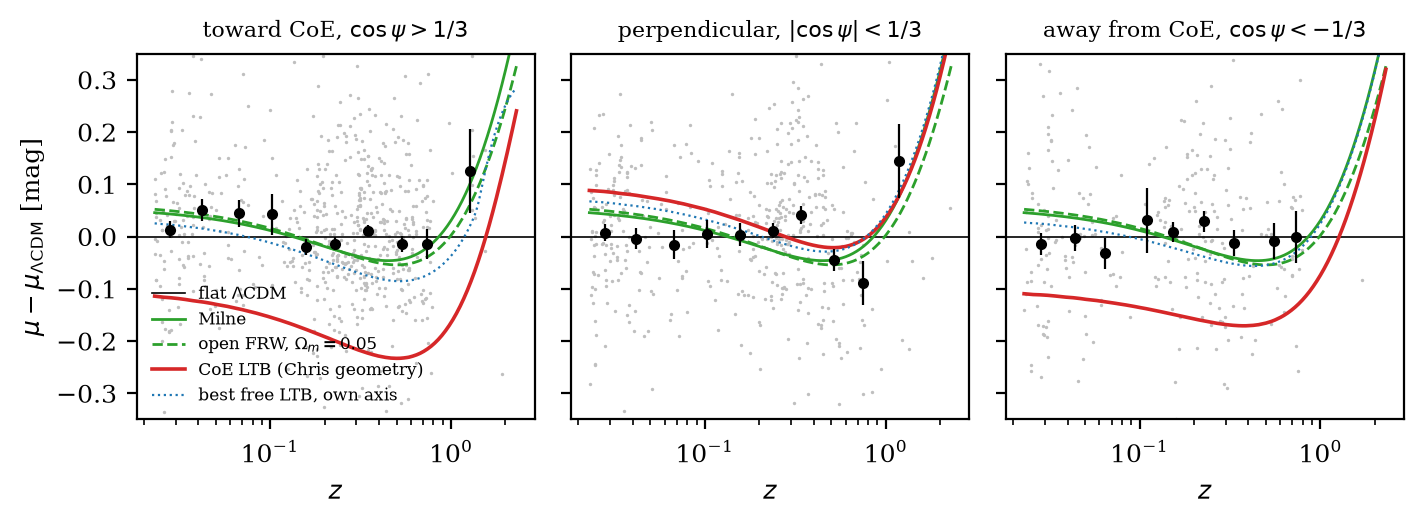
\includegraphics[width=\textwidth]{fig_hubble_resid.png}
\caption{Pantheon+ distance moduli relative to flat $\Lambda$CDM, split by the angle $\psi$ between each SN and the CoE. Grey points are individual SNe and black points are inverse-variance binned means with diagonal errors, for display only. The curves are Milne (solid green), the baryons-only open universe (dashed green), your CoE geometry evaluated along the bin's central direction (red), and the best free LTB model along its own axis (dotted blue). Each model uses its own best-fit offset.}\label{fig:hub}
\end{figure*}

\section{What the geometry explains}\label{sec:mig}
In Migkas's convention the cluster normalisation scales as $A\propto H_0^2$, so we model it as
\begin{equation}\label{eq:A}
\frac{A(\ell)}{\langle A\rangle}=\frac{D_L^{-2}(z=0.1,\ell,b=0)}{\big\langle D_L^{-2}\big\rangle}
\end{equation}
and compare with the digitised $A(\ell)$ profile, using a free normalisation and diagonal errors. Table~\ref{tab:mig} gives the results. Your geometry on the CoE axis improves strongly on isotropy and follows the data closely, with the maximum of $A$ on the axis as the corrected sign requires. Adding a baryons-only background keeps almost all of that improvement. Pointing the same mass away from the CoE, toward the axis that the SNe alone would pick, destroys the cluster fit, so the clusters fix the axis. A joint fit to both data sets over $L/D$, $m_c$ and the axis lands close to the CoE, slightly below the Galactic plane, with a lump broader and slightly lighter than yours (Table~\ref{tab:par}). It keeps most of the cluster improvement and fits the SNe slightly better than Milne. The SNe also constrain the background. With $\Omega$ free and the CoE mass on the CoE axis, the fit returns a density close to the baryon value (Table~\ref{tab:fits}), which means about zero dark matter, and $\Lambda$CDM-equivalent matter is disfavoured.

The cluster $\chi^2$ values overstate the evidence, because the digitised points come from overlapping sliding cones and are strongly correlated. The comparison between rows is more reliable than the absolute numbers.




\begin{figure*}[t]\centering
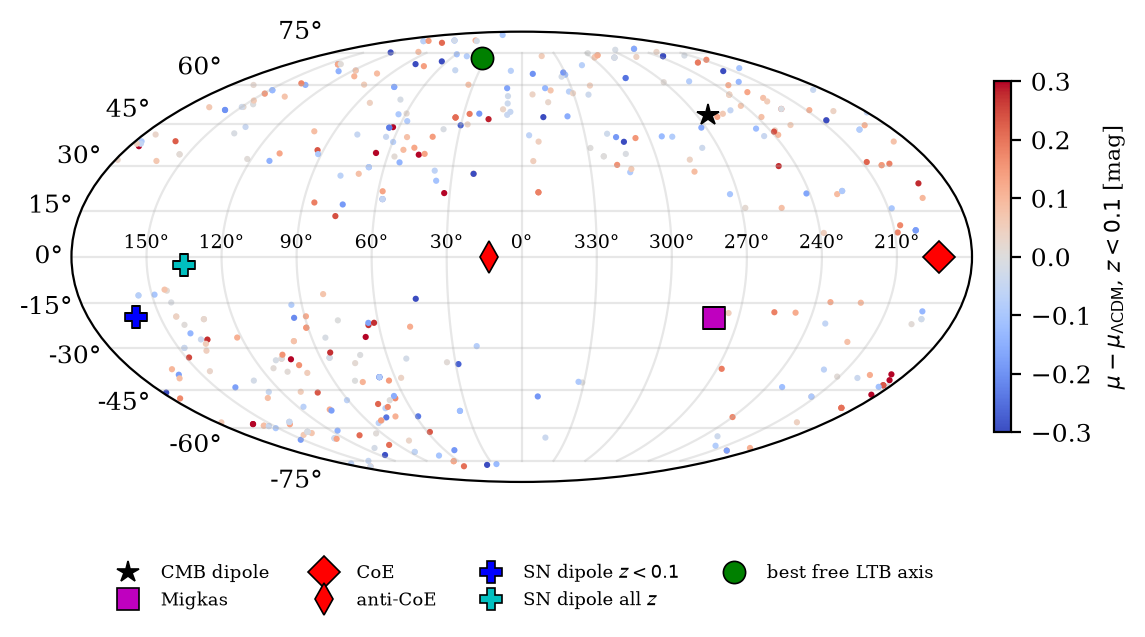
\includegraphics[width=0.62\textwidth]{fig_sky.png}
\caption{Galactic Mollweide map (longitude increasing to the left) of $\Lambda$CDM residuals for $z_{\rm HD}<0.1$, with the CMB dipole (also the axis tested by Colin et al.\ \cite{Colin2019}), the Migkas cluster axis, the CoE and anti-CoE, the $\Lambda$CDM residual dipoles, and the best free LTB axis.}\label{fig:sky}
\end{figure*}

\section{Supernova fit quality in context}\label{sec:fits}
Table~\ref{tab:fits} lists the SN $\chi^2$ of every model, with flat $\Lambda$CDM as a reference point. $\Lambda$CDM has had decades of calibration against these data, and the Pantheon+ standardisation was itself built within it, so the differences are context for a toy model and not a verdict. Every $\Lambda=0$ model, including Milne and the open baryons-only Friedmann model, sits at a similar distance from $\Lambda$CDM. That gap is in the sky-averaged distance--redshift relation. The toy model decelerates by construction, and we do not add anything to change that.

Within the $\Lambda=0$ family the ordering is informative. Your CoE mass with a baryons-only background fits much better than the same mass with no background or with $\Lambda$CDM-equivalent matter, and a free background settles near the baryon density. The best free LTB model is close to Milne. Freeing the axis in the SN-only fits moves it away from the CoE, where the lump mainly shifts the overall distance scale, but that axis loses the cluster signal (Table~\ref{tab:mig}).

Two degeneracies control the free fits. At fixed $m_c$ and $L/D$ the $\chi^2$ hardly depends on $D$, because the tidal field at the observer scales as $GM/D^3\propto m_cH_0^2$. The background density goes to its lower bound whenever the lump is free. Figure~\ref{fig:hub} shows the data split by angle from the CoE. The open models differ from $\Lambda$CDM mainly in the redshift dependence common to all bins. Your exact geometry adds the quadrupole that produces the cluster signal, and the binned SNe do not show it at that amplitude. The broader joint-fit geometry has a weaker quadrupole at high redshift, which is why it fits the SNe about as well as Milne while keeping most of the cluster signal.



\begin{table}[htbp]\centering\footnotesize
\caption{LTB geometries. $D$ is in the geometric units of the previous note, $m_c$ follows Eq.~(\ref{eq:mc}), $(\ell_0,b_0)$ is the lump axis, $\theta_{\rm CoE}$ its angle from the CoE, and $\chi^2$ the SN value for $z_{\rm HD}>0.023$.}\label{tab:par}
\setlength{\tabcolsep}{2.5pt}
\resizebox{\columnwidth}{!}{\begin{tabular}{@{}lrrrrrrrr@{}}\toprule
Geometry & $D$ & $L/D$ & $m_c$ & $\Omega$ & $\ell_0$ & $b_0$ & $\theta_{\rm CoE}$ & $\chi^2$\\\midrule
\tabinput{tab_par.tex}
\bottomrule\end{tabular}}\end{table}




\section{Direction tests}
We also looked for anisotropy in the SN residuals without assuming a model. We fit a dipole to the residuals from each model with the full covariance,
\begin{equation}\label{eq:dip}
m_{b,{\rm corr},i}-\mu_{\rm model}(z_i)=\mathcal M+\mathbf d\cdot\hat{\mathbf n}_i ,
\end{equation}
and we repeat the redshift-dependent deceleration test of Colin et al.\ \cite{Colin2019},
\begin{equation}\label{eq:colin}
q_0(\hat{\mathbf n})=q_m+q_d\,(\hat{\mathbf n}\cdot\hat{\mathbf c})\,e^{-z/S},\qquad S=0.0262,
\end{equation}
together with a simple split into hemispheres. Tables~\ref{tab:dip} and~\ref{tab:q} give the results, and Fig.~\ref{fig:sky} shows the residual map.

The only residual dipole with modest significance is in the lowest redshift bin, and its axis lies between the CoE and the Galactic anticentre direction. The higher redshift bins show nothing coherent. With the Colin parametrisation, a CMB-dipole axis gives a positive $q_d$, the Migkas axis gives nothing, and the CoE axis gives a negative $q_d$, meaning a smaller apparent deceleration parameter toward the CoE. None of these is significant, and the sign found by Colin et al.\ is not reproduced once Pantheon+ uses corrected redshifts. The hemisphere values agree within their errors for every axis. The low-$z$ dipole is also the regime most sensitive to the flow model behind $z_{\rm HD}$, so we treat it as a hint and not as a detection. Its axis is closer to the CoE than to any other tested axis. The LTB lump produces mainly a quadrupole, so this alignment is suggestive rather than a prediction. The SN residuals show nothing that conflicts with the CoE axis.

\begin{table}[htbp]\centering\footnotesize
\caption{Residual dipoles from Eq.~(\ref{eq:dip}) with the full covariance. $A$ is the dipole amplitude in magnitudes (positive means more distant than the model), $\delta\theta_{68}$ the 68\% direction uncertainty, $\theta_{\rm CoE}$ the angle from the CoE, and $\Delta\chi^2$ the improvement over no dipole for three extra parameters.}\label{tab:dip}
\setlength{\tabcolsep}{2.2pt}
\resizebox{\columnwidth}{!}{\begin{tabular}{@{}lrrrrrrrr@{}}\toprule
Residuals & $N$ & $A$ & $\sigma_A$ & $\ell$ & $b$ & $\delta\theta_{68}$ & $\theta_{\rm CoE}$ & $\Delta\chi^2$\\\midrule
\tabinput{tab_dip.tex}
\bottomrule\end{tabular}}\end{table}

\begin{table}[htbp]\centering\footnotesize
\caption{Deceleration-parameter anisotropy from the cosmographic expansion with $z<0.8$. Columns 3--6 are the fit of Eq.~(\ref{eq:colin}) with $j_0$ free, and $\Delta\chi^2$ is its improvement over $q_d=0$. The last four columns give $q_0$ with $j_0=1$ in the hemisphere toward the axis and in the opposite one. The last axis is the $\Lambda$CDM residual dipole of Table~\ref{tab:dip}, so its $\Delta\chi^2$ carries a look-elsewhere penalty.}\label{tab:q}
\setlength{\tabcolsep}{1.6pt}
\resizebox{\columnwidth}{!}{\begin{tabular}{@{}llrrrrrrrr@{}}\toprule
$z_{\rm min}$ & Axis & $q_m$ & $q_d$ & $\sigma_{q_d}$ & $\Delta\chi^2$ & $q_0^{\rm tow}$ & $\sigma$ & $q_0^{\rm away}$ & $\sigma$\\\midrule
\tabinput{tab_q.tex}
\bottomrule\end{tabular}}\end{table}




\section{Ages}
All $\Lambda=0$ models without dark matter have ages comparable to the oldest globular clusters, which are 12--13 Gyr old, when $H_0=70$. Adding $\Lambda$CDM-equivalent matter, or using $H_0=73$, pushes the lump models below that range (Table~\ref{tab:fits}). The age is therefore not a strong discriminant for the baryons-only models, and it counts against the model with $\Lambda$CDM-equivalent matter.


\section{Caveats}
The $z_{\rm HD}$ redshifts include peculiar-velocity corrections computed from a flow model built in $\Lambda$CDM, and those corrections contain part of the nearby anisotropy we are testing. The low-$z$ dipole and the cluster comparison are the parts most affected. The Pantheon+ standardisation and systematics were built in a $\Lambda$CDM framework. The models are gravity-only dust with $\Lambda=0$, as the toy model intends. The cluster profile is a digitised figure with correlated points, and we use only the $b=0$ ring. The free-LTB search used several Nelder--Mead starts on a nearly flat surface, so its optimum is shallow, although the conclusion does not depend on its exact location.


\section{Conclusion}
The CoE geometry does what it was built to do. On the CoE axis it lowers the cluster $\chi^2$ from 44.7 for isotropy to 20.3 (Table~\ref{tab:mig}), with the $m=2$ shape, axis and corrected sign $A\propto H_0^2$ that general relativity confirms. A joint cluster and SN fit puts the axis $16^\circ$ from the CoE. The SNe prefer a background near the baryon density, $\Omega\approx0.068$, so the data favour the zero-dark-matter version of the model, and baryons only is the preferred physical case. The shell theorem makes the ingredients explicit. For the instantaneous field only a positive net mass inside $D-R$ matters, although the integrated history can override this, and uniform matter around the visible sphere or symmetric matter beyond $D+R$ does not change the pattern. The SN residuals contain no significant anisotropy that conflicts with the CoE axis. Flat $\Lambda$CDM fits the sky-averaged SN distances better (Table~\ref{tab:fits}), which is context for a gravity-only, always-decelerating toy model and not a verdict on it.

\begin{thebibliography}{99}\scriptsize\setlength{\itemsep}{0pt}
\bibitem{Migkas2020} K.~Migkas et al., A\&A 636, A15 (2020).
\bibitem{Migkas2021} K.~Migkas et al., A\&A 649, A151 (2021).
\bibitem{Scolnic2022} D.~Scolnic et al., ApJ 938, 113 (2022).
\bibitem{Brout2022} D.~Brout et al., ApJ 938, 110 (2022).
\bibitem{Bondi1947} H.~Bondi, MNRAS 107, 410 (1947).
\bibitem{Bolejko2011} K.~Bolejko, M.-N.~C\'el\'erier, A.~Krasi\'nski, Class.\ Quantum Grav.\ 28, 164002 (2011).
\bibitem{Colin2019} J.~Colin, R.~Mohayaee, M.~Rameez, S.~Sarkar, A\&A 631, L13 (2019).
\end{thebibliography}
\end{document}
